\documentclass[11pt]{article}
\usepackage[T1]{fontenc}
\usepackage{lmodern}
\usepackage{parskip}
\usepackage[colorlinks=true,urlcolor=Blue,linkcolor=black,citecolor=black]{hyperref}
\usepackage{graphicx}
\usepackage{amsmath}
\usepackage[utf8]{inputenc}
\usepackage[spanish]{babel}
\usepackage{fancyhdr}
\usepackage{csquotes}
\usepackage{lastpage}
\usepackage{array}
\usepackage{listings}
\usepackage{color}
\definecolor{dkgreen}{rgb}{0,0.6,0}
\definecolor{gray}{rgb}{0.5,0.5,0.5}
\definecolor{mauve}{rgb}{0.58,0,0.82}
\usepackage[affil-it]{authblk}
\usepackage[activate={true,nocompatibility},final,tracking=true,kerning=true,spacing=true,factor=1100,stretch=10,shrink=10]{microtype}
\usepackage[hmargin=2cm,top=4cm,headheight=65pt,footskip=65pt]{geometry}
\usepackage{hyperref}
\usepackage{graphicx}
\usepackage{float}
\graphicspath{ {./screenshots/p02/} }

% Documento
\begin{document}

% Título
\title{IFA. Práctica de laboratorio 02}

\author{Hugo Fonseca Díaz \\ email \href{mailto:uo258318@uniovi.es}{uo258318@uniovi.es}}
\affil{Escuela de Ingeniería Informática. Universidad de Oviedo.}

\maketitle

% Ejercicio 1
\section{Ejercicio 1}
Se guarda la fecha y hora del sistema en el archivo \verb|ej01.txt| con el comando \verb|date > ej01.txt|. Se muestra ese archivo con el comando \verb|cat|.

\begin{figure}[H]
  \caption{Ejercicio 1: Resultado del comando \textit{cat ej01.txt}.}
  \centering
  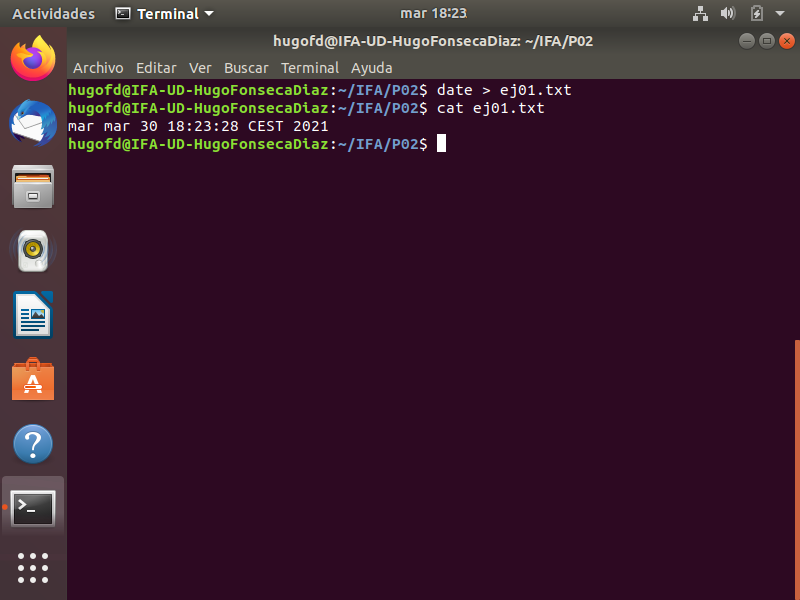
\includegraphics{e1-1.png}
\end{figure}

Se accede al sitio web \url{https://time.is/es/Spain} y se comprueba que la hora es la misma.

\begin{figure}[H]
    \caption{Ejercicio 1: Hora en el sitio web \textit{time.is}.}
  \centering
  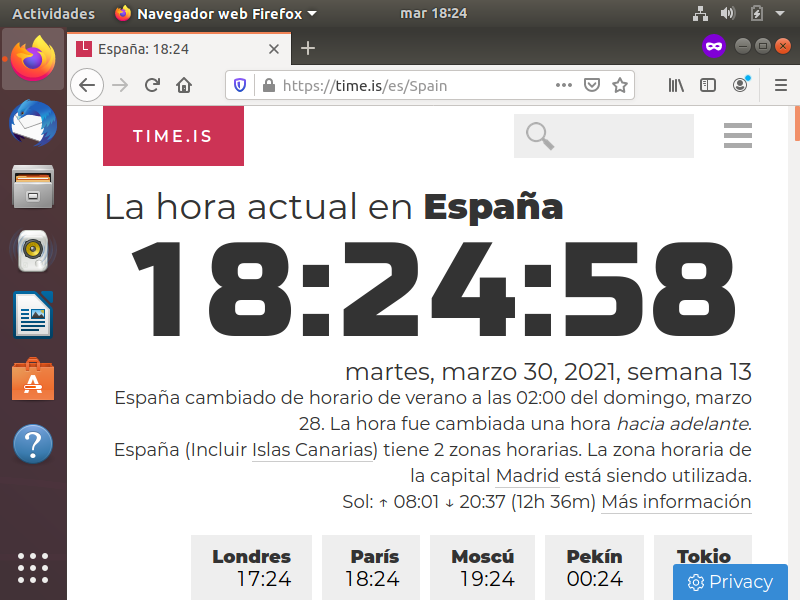
\includegraphics{e1-2.png}
\end{figure}

% Ejercicio 2
\section{Ejercicio 2}
Se utiliza el comando \verb|uname| con las opciones \verb|v| (lista la versión del kernel) y \verb|o| (lista el nombre del sistema operativo).

\begin{figure}[H]
    \caption{Ejercicio 2: \textit{uname -vo}.}
  \centering
  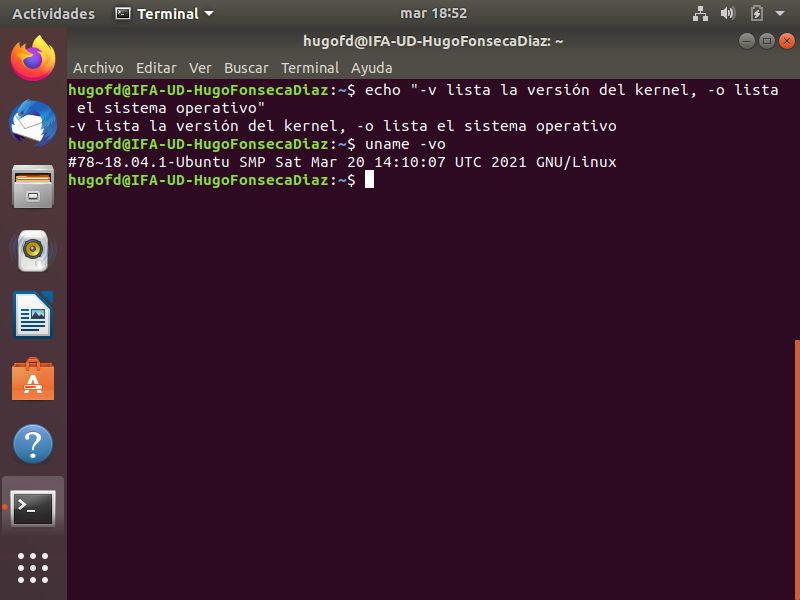
\includegraphics{e2.png}
\end{figure}

% Ejercicio 3
\section{Ejercicio 3}
Se utiliza el comando \verb|lshw|, primero con la flag \verb|short| para encontrar el nombre de la clase de los dispositivos de red.

\begin{figure}[H]
    \caption{Ejercicio 3: \textit{lshw -short}.}
  \centering
  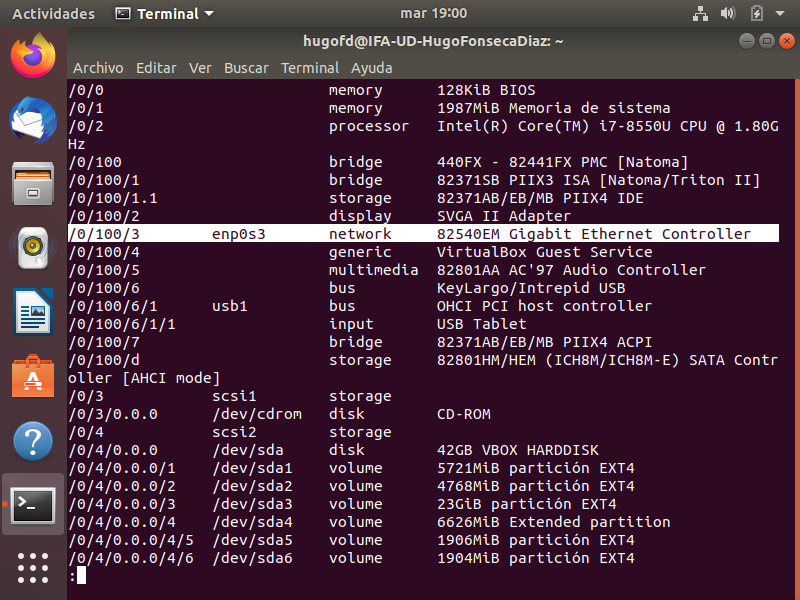
\includegraphics{e3-1.png}
\end{figure}

Una vez se sabe que el nombre de la clase de los dispositivos de red es \verb|network|, se utiliza el comando \verb|lshw| con la flag \verb|-class network|.

\begin{figure}[H]
    \caption{Ejercicio 3: \textit{lshw -class network}.}
  \centering
  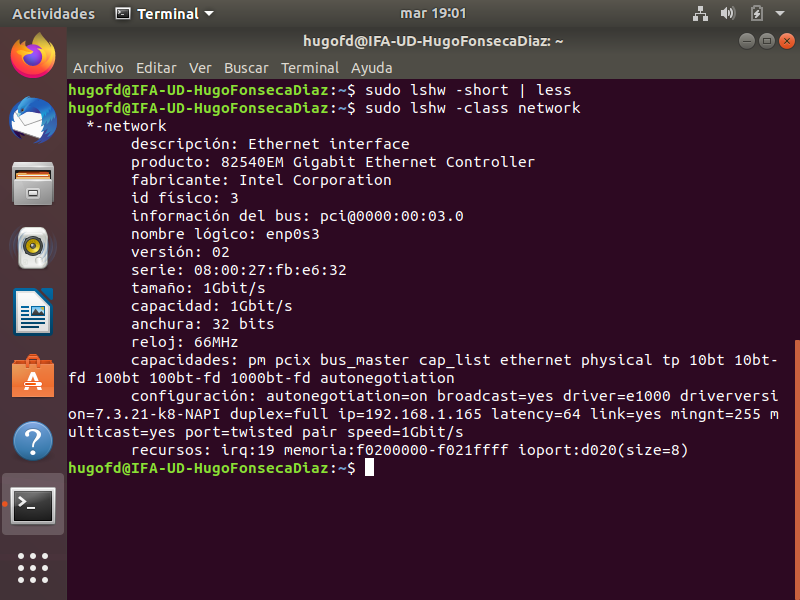
\includegraphics{e3-2.png}
\end{figure}

También puede utilizarse el comando \verb|ip -h a| para mostrar más información sobre el dispositivo de red \verb|enp0s3|.

\begin{figure}[H]
    \caption{Ejercicio 3: \textit{ip -h a}.}
  \centering
  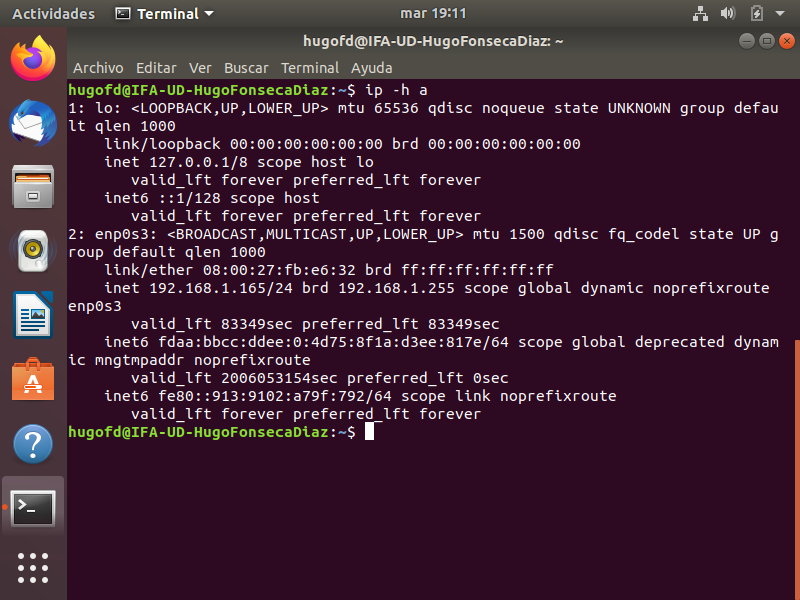
\includegraphics{e3-3.png}
\end{figure}

% Ejercicio 4
\section{Ejercicio 4}
Se utiliza el comando \verb|netstat| del paquete \verb|net-tools|. Su flag \verb|a| permite ver todos los sockets, por lo que \verb|sudo netstat -a > ej04.txt| guarda la información de los sockets activos y no activos en un fichero de texto. También son interesantes sus flags \verb|n| (se muestran las direcciones numéricamente), \verb|p| (se muestran los procesos pertenecientes a los sockets), \verb|t| (tcp) y \verb|u| (udp).

\begin{figure}[H]
    \caption{Ejercicio 4: \textit{cat ej04.txt | less}.}
  \centering
  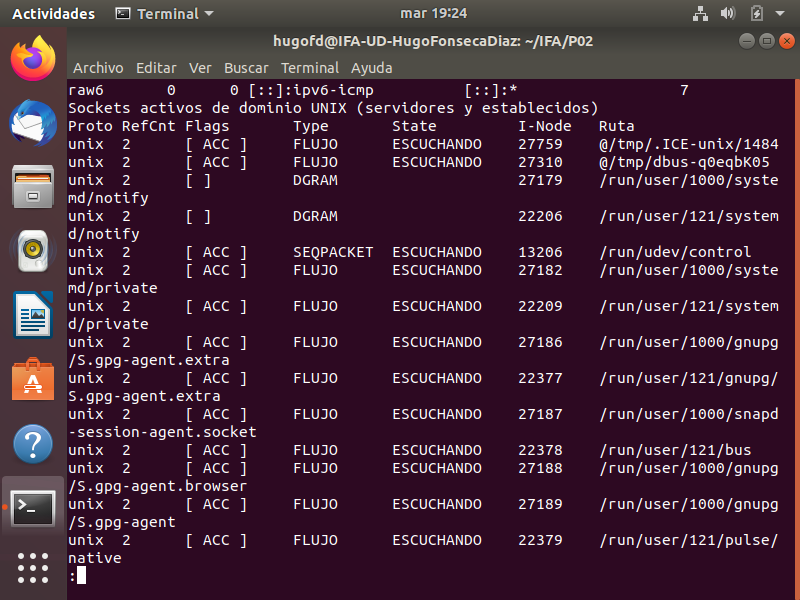
\includegraphics{e4-1.png}
\end{figure}

\begin{figure}[H]
    \caption{Ejercicio 4: \textit{sudo netstat -ptun}.}
  \centering
  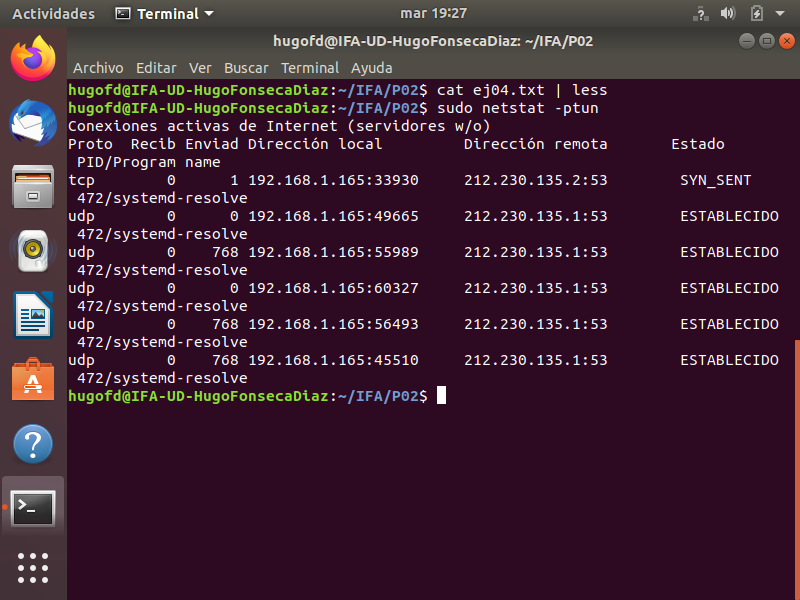
\includegraphics{e4-2.png}
\end{figure}

También se puede ver información de los servicios de red en \verb|/etc/services|.

\begin{figure}[H]
    \caption{Ejercicio 4: \textit{less /etc/services}.}
  \centering
  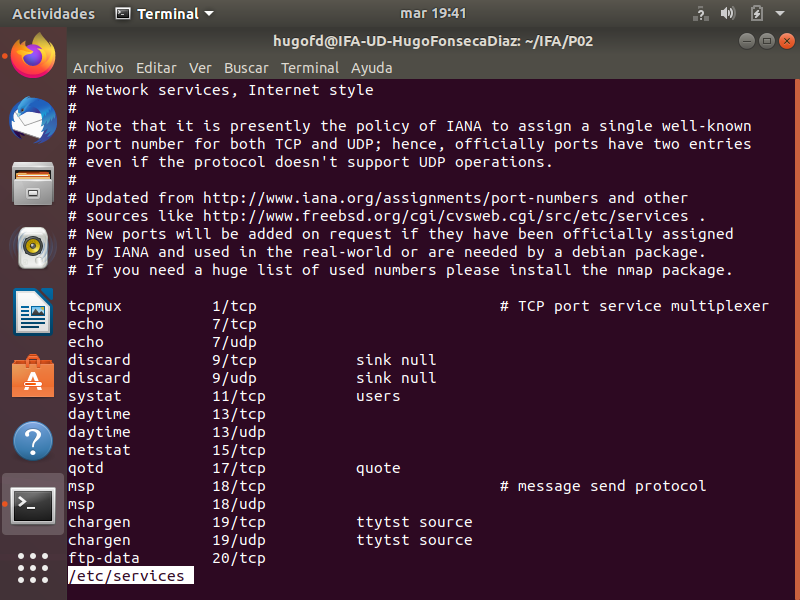
\includegraphics{e4-3.png}
\end{figure}

% Ejercicio 5
\section{Ejercicio 5}
Para resolver este ejercicio se usan tres comandos: \verb|who| muestra los usuarios conectados y la terminal en la que están, \verb|tty| muestra la terminal conectada actualmente al standard input y \verb|uptime| muestra el tiempo que ha pasado desde el arranque del sistema.

\begin{figure}[H]
    \caption{Ejercicio 5: \textit{who, tty} y \textit{uptime}.}
  \centering
  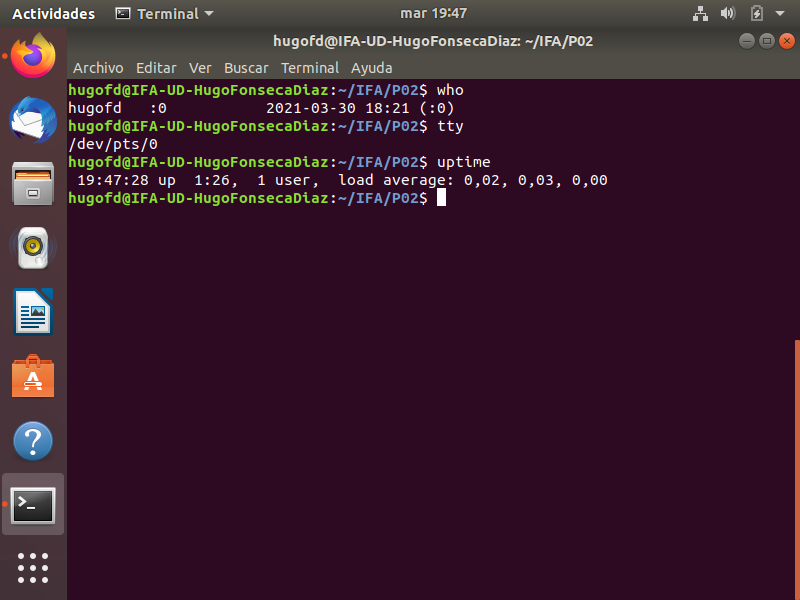
\includegraphics{e5.png}
\end{figure}

% Ejercicio 6
\section{Ejercicio 6}
Existen al menos dos opciones de mostrar la información sobre la tabla de enrutamiento: mediante el comando \verb|netstat| con su flag \verb|r| (que muestra la tabla de enrutamiento) o usando el comando \verb|route| con su flag \verb|n| (que muestra las direcciones de red de forma numérica).

\begin{figure}[H]
    \caption{Ejercicio 6: \textit{netstat -r} y \textit{route -n}.}
  \centering
  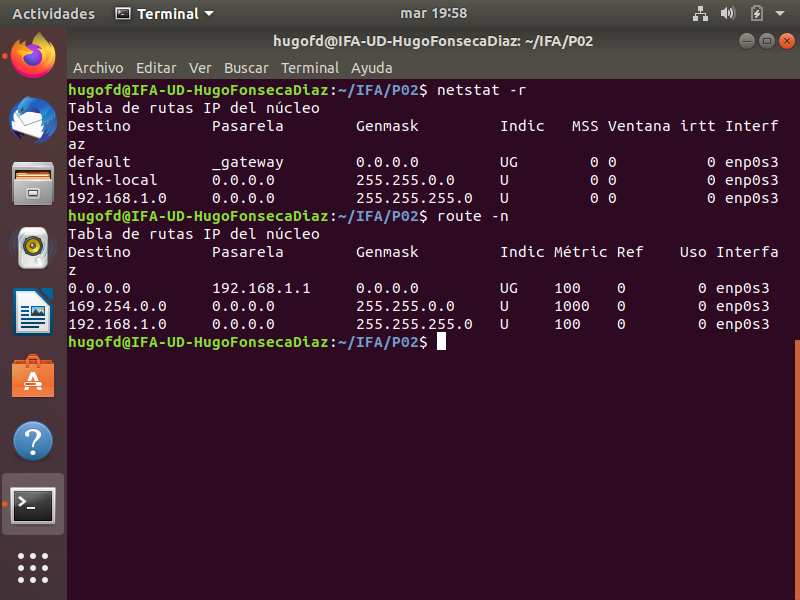
\includegraphics{e6.png}
\end{figure}

% Ejercicio 7
\section{Ejercicio 7}
Se usa el comando \verb|ps|. Dicho comando puede utilizarse siguiendo tres sintaxis: la de UNIX, la de BSD o la de GNU. Para mostrar todos los procesos del sistema con sintaxis de UNIX podría usarse \verb|ps -eF|. Con sintaxis de BSD se puede usar \verb|ps axu|. Para que se muestre el nombre del proceso sin cortarse se puede pasar el resultado del comando \verb|ps| al comando \verb|less| con una pipe de UNIX.

\begin{figure}[H]
    \caption{Ejercicio 7: \textit{ps axu | less}.}
  \centering
  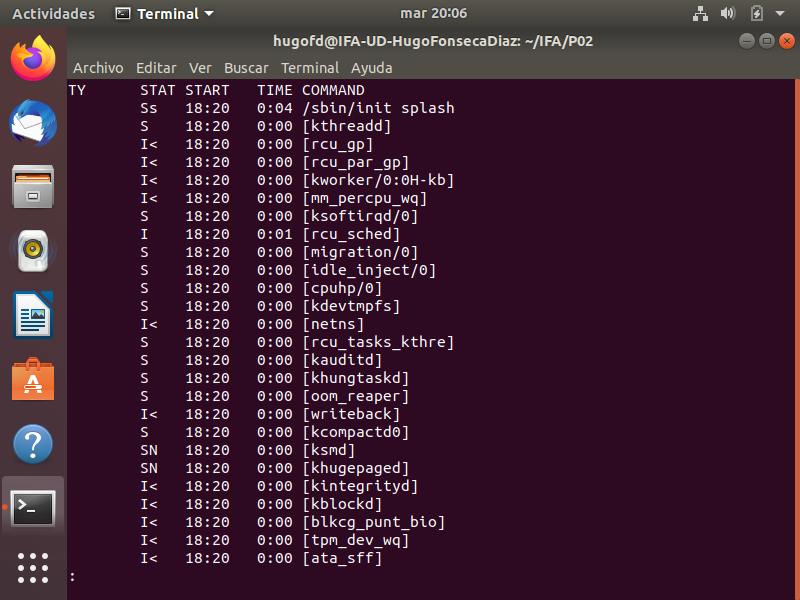
\includegraphics{e7.png}
\end{figure}

% Ejercicio 8
\section{Ejercicio 8}
Se usarán los comandos \verb|last| y \verb|lastb|. El primero se utiliza para sacar la información de los accesos de todos los usuarios al sistema, incluyendo también un ejemplo de uso para un usuario concreto. El segundo es un comando similar pero buscando en \textit{/var/log/btmp}, lo que muestra intentos fallidos de acceso al sistema.

\begin{figure}[H]
    \caption{Ejercicio 8: \textit{last} y \textit{lastb}.}
  \centering
  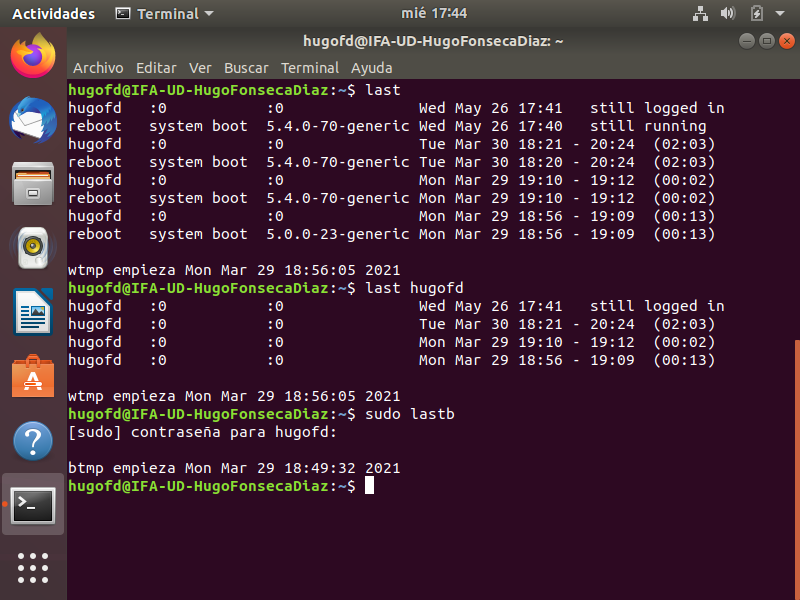
\includegraphics{e8.png}
\end{figure}

% Ejercicio 9
\section{Ejercicio 9}
Se utiliza el comando \verb|lsof|, cuya salida está pensada para ser la entrada de otro programa que la parsee. Se hace una pipe de Unix con el comando \verb|less| para poder visualizar la salida del comando.

\begin{figure}[H]
    \caption{Ejercicio 9: \textit{lsof | less}.}
  \centering
  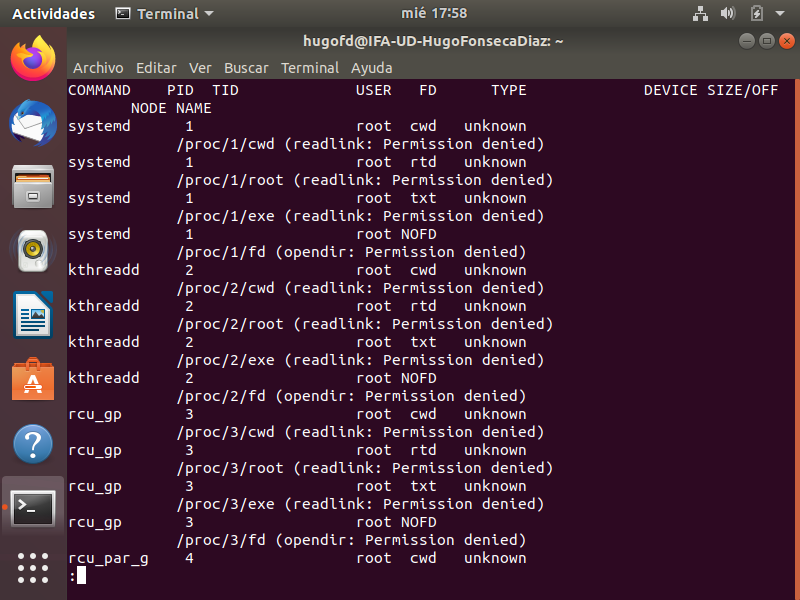
\includegraphics{e9.png}
\end{figure}

% Ejercicio 10
\section{Ejercicio 10}
Se puede usar el comando \verb|lsblk| con la opción \verb|f|. El comando muestra información de los dispositivos del sistema y la opción \textit{f} muestra los sistemas de ficheros de los mismos.

\begin{figure}[H]
    \caption{Ejercicio 10: \textit{lsblk -f}.}
  \centering
  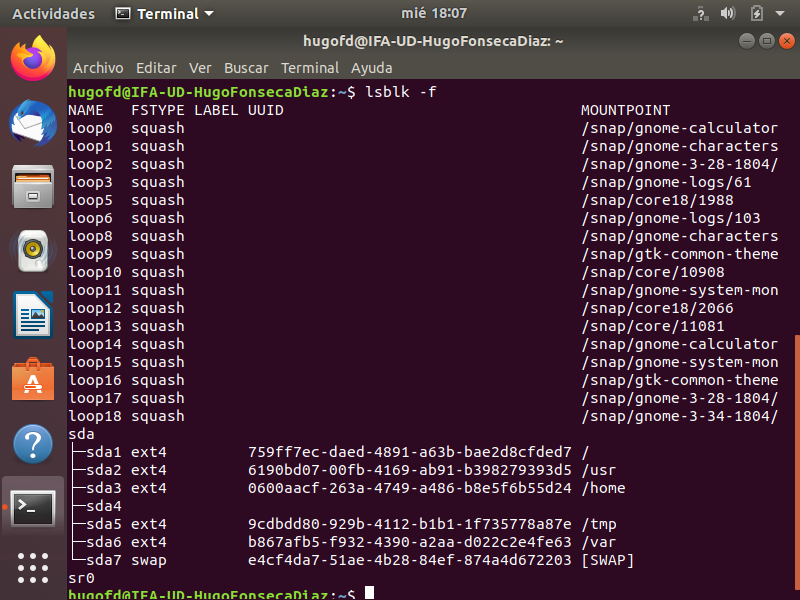
\includegraphics{e10.png}
\end{figure}

% Ejercicio 11
\section{Ejercicio 11}
Para mostrar las particiones del disco \textit{sda} junto a sus sectores de inicio y fin, se utiliza el comando \verb|fdisk| con la opción \verb|l|, que lista dichas particiones, y pasándole como parámetro el disco que queremos inspeccionar (en este caso \textit{/dev/sda}). No es necesario especificarle que las unidades del tamaño sean sectores puesto que es el comportamiento por defecto.

\begin{figure}[H]
    \caption{Ejercicio 11: \textit{sudo fdisk -l /dev/sda}.}
  \centering
  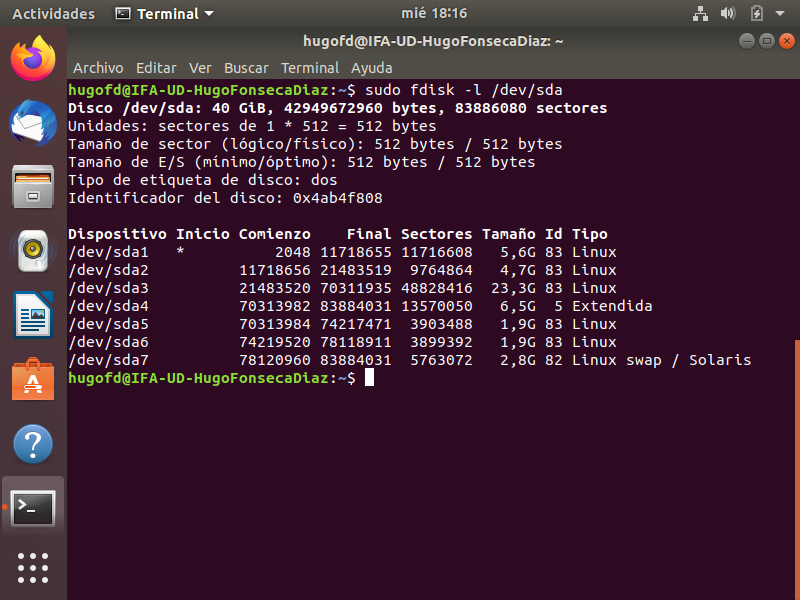
\includegraphics{e11.png}
\end{figure}

% Ejercicio 12
\section{Ejercicio 12}
El fichero donde el kernel almacena las acciones realizadas por \verb|cron| se encuentra en \textit{/var/log/syslog}. Puede hacerse un \verb|grep| con la string \textit{cron} en dicho archivo para visualizar las acciones, sin embargo, debido al poco espacio en la partición \textit{/var}, en nuestro caso ese archivo está vacío.

\begin{figure}[H]
    \caption{Ejercicio 12: \textit{grep cron /var/log/syslog}.}
  \centering
  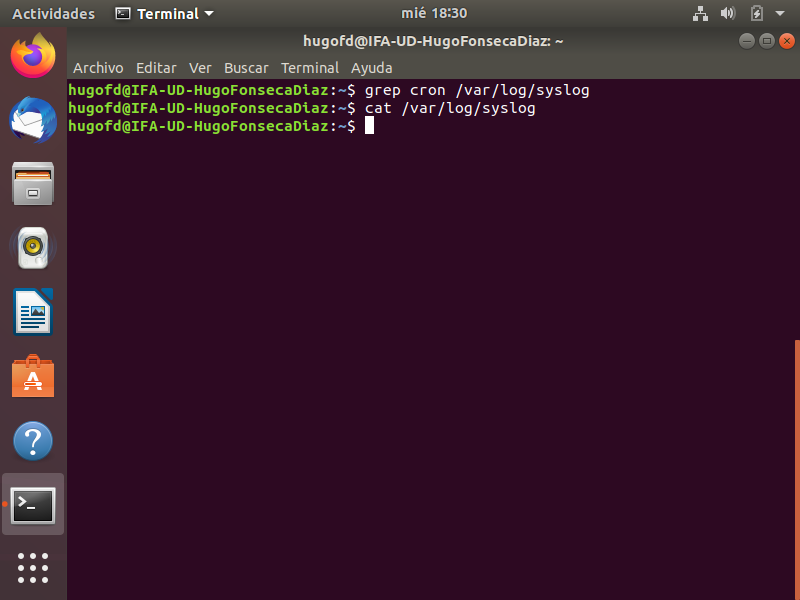
\includegraphics{e12.png}
\end{figure}

% Ejercicio 24
\section{Ejercicio 24}
El historial de comandos de \verb|bash| del usuario se encuentra en un fichero oculto de su carpeta \textit{HOME} llamado \textit{bash\_history}. Se puede  utilizar el comando \verb|ls| con la flag \textit{a} para listar todos los archivos, incluidos los ocultos, para comprobar que efectivamente existe el archivo del historial.

\begin{figure}[H]
    \caption{Ejercicio 24: \textit{ls -a; cat .bash\_history}.}
  \centering
  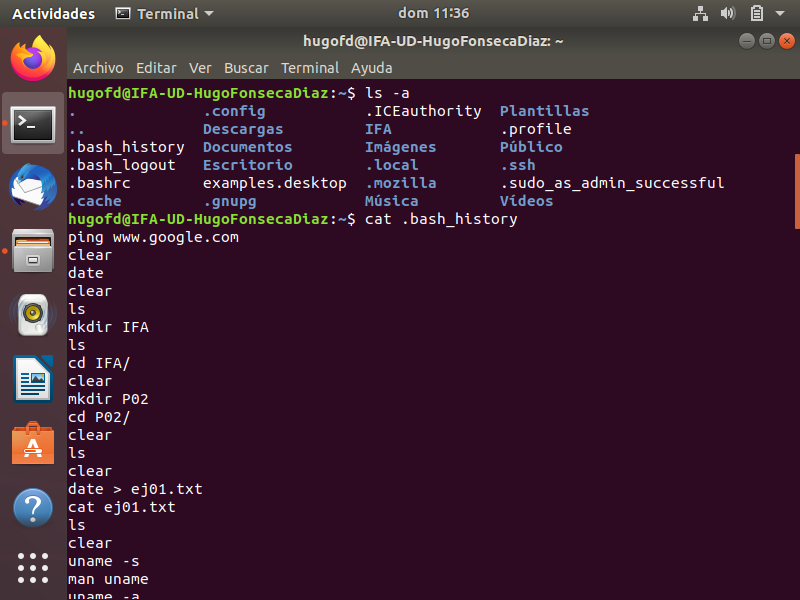
\includegraphics{e24.png}
\end{figure}

% Ejercicio 27
\section{Ejercicio 27}
Se descomprime el archivo con el comando \verb|tar| y las flags \textit{xvzf}, siendo \textit{x} una indicación de que se quiere extraer los contenidos del archivo comprimido, \textit{v} para que lo haga de manera verbosa, \textit{z} para indicarle al comando que el archivo es un zip y \textit{f} para pasarle el fichero que se desea extraer al comando.

\begin{figure}[H]
    \caption{Ejercicio 27: \textit{tar -xvzf}.}
  \centering
  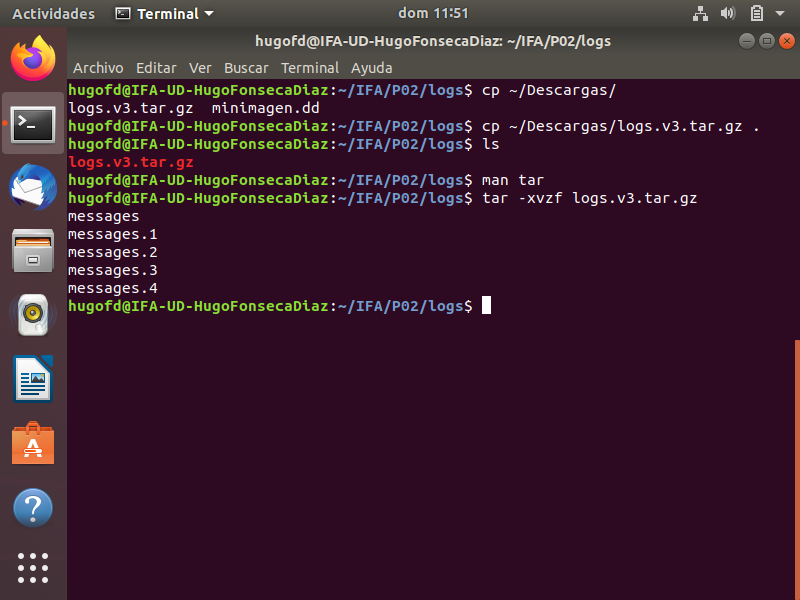
\includegraphics{e27-1.png}
\end{figure}

Una vez descomprimidos los ficheros de texto, se procede a utilizar tres nuevas herramientas. Se usa \verb|tac| para concatenar ficheros de forma inversa (es el comando \verb|cat| invertido), el lenguaje de programación AWK para procesar texto y el comando \verb|uniq| para omitir líneas repetidas.

\begin{figure}[H]
    \caption{Ejercicio 27: \textit{tac, AWK y uniq}.}
  \centering
  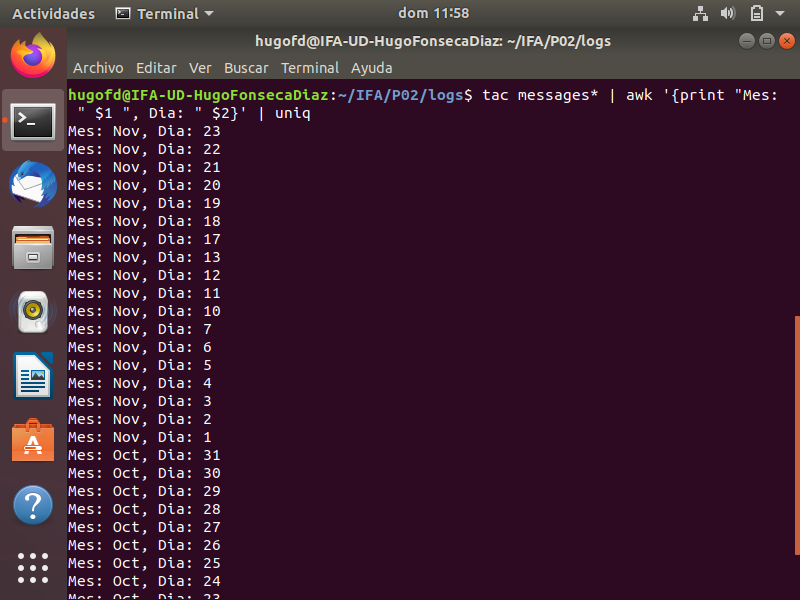
\includegraphics{e27-2.png}
\end{figure}

% Ejercicio 28
\section{Ejercicio 28}
Se usan los comandos \verb|tac| y \verb|grep|. El primero se usa para concatenar inversamente los ficheros de los mensajes y el segundo para buscar las líneas donde aparece la cadena de texto \textit{"Nov 13"}.

\begin{figure}[H]
    \caption{Ejercicio 28: \textit{tac y grep}.}
  \centering
  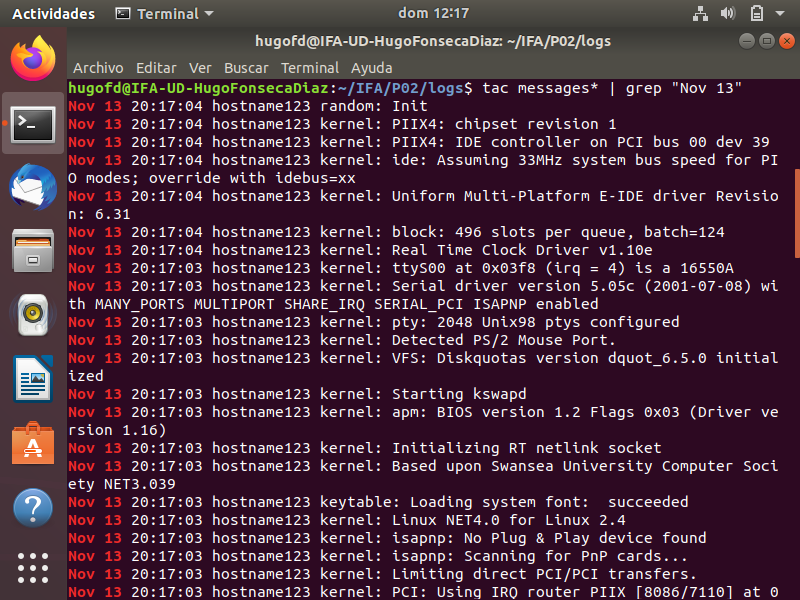
\includegraphics{e28.png}
\end{figure}

% Ejercicio 29
\section{Ejercicio 29}
Se usan tres herramientas. La primera es \verb|tac|, para concatenar inversamente los ficheros de los mensajes. La segunda es \verb|grep|, para buscar entre los mensajes aquellos con la string indicada por el enunciado. Por último, se utiliza el lenguaje de procesado de textos AWK para printear las columnas deseadas, en este caso con un título indicativo.

\begin{figure}[H]
    \caption{Ejercicio 29: \textit{tac, grep y awk}.}
  \centering
  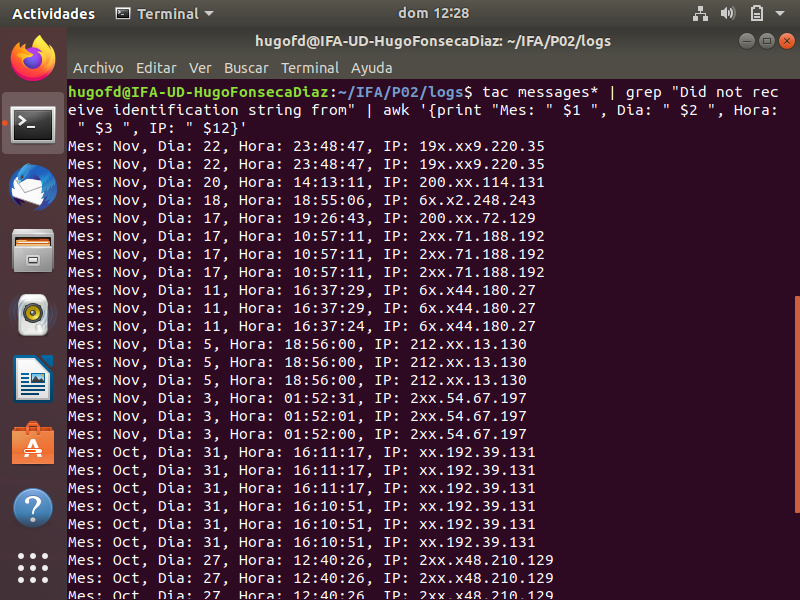
\includegraphics{e29.png}
\end{figure}

% Bibliografía
\begin{thebibliography}{8}
\end{thebibliography}

\end{document}


